\documentclass[a4paper,14pt]{article}

\usepackage{amsmath,amsfonts,amssymb,amsthm,epsfig,epstopdf,titling,url,array}
\usepackage[utf8x]{inputenc}
\usepackage[russian]{babel}
%\usepackage[T2A]{fontenc}
\usepackage{amsmath,amssymb,amsthm,amscd,amsfonts,graphicx}
\usepackage[14pt]{extsizes}

\usepackage{cleveref}
\usepackage{tikz}
\usetikzlibrary{arrows,shapes,snakes,automata,backgrounds,petri}

\newcommand{\workflow}{\textit{workflow}}
\newenvironment{definition}[1]{
\hskip \labelsep {\bfseries #1} \it}

\newtheorem{theorem}{Теорема}
\newtheorem{lemma}{Лемма}
\newtheorem{corollary}{Вывод}



\begin{document}
\textwidth 15.5cm
\topmargin -1cm
\parindent 1cm
\textheight 24cm
\parskip 1.5mm



\section{Введение}
\subsection*{Цель работы}
Целью работы являляется построение модели workflow, ориентированного  на решение научно-инженерных задач в распределённой среде. И разработка методов и инструментов анализа этой модели.
 Под инженерными и научными задачами в данном контексте мы понимаем 
мультидисциплинарные задачи в форме так называемых композитных приложений. В работе мы рассматриваем примеры задач обработки и анализа данных, например построения  суррогатных моделей , и задач многодисциплинарной оптимизации. Наиболее распространенным подходом к представлению таких композитных приложений является формализм потока работ, или workflow.

Под workflow подразумевается формальное представление (модель) некоторого процесса, включающее в себя:
\begin{enumerate}
\item[-] Описание операций, из которых состоит процесс.
\item[-] Описание исполнителей, которые выполняют указанные операции.
\item[-] Описание зависимостей между операциями, а именно :
\begin{enumerate}
\item[•] потоков управления, которые определяют последовательность выполнения операций 
\item[•] потоков данных, которые
определяют передачу информации между исполнителями.
\end{enumerate}
\end{enumerate}


Для выполнения задач, поставленных с помощью workflow, требуется система управления или исполнения( Workflow Managment system, WFMS)).Обычно WFMS состоит из набора программных
компонентов, предназначенных для:
\begin{enumerate}
\item[•] хранения и интерпретации описаний
процессов 
\item[•] создания и управления экземплярами запущенных процессов
\item[•] организации их взаимодействия с участниками
процесса и внешними приложениями.
\end{enumerate}



\subsection*{Отличие научных workflow от бизнес-процессов}
  Исторически данный подход широко использовался для описания бизнес-процессов.Однако в данной работе мы рассматриваем научно-инженерные задачи, приведём их некоторые характерные особенности:
 
\begin{enumerate}
\item[-] Научно-инженерные задачи требуют существенных вычислительных затрат.
\item[-] Научно-инженерные задачи работаютт с большими объёмами данных.
\item[-] Зачастую бывает  необходимо одинаковым образом обрабатывать разные наборы данные.
\item[-]  Ввиду перечисленных выше трёх пунктов, задачи согут быть ресурсоёмеими, поэтому имеет смысл использовать распределённую вычислительную среду.
\item[-]  характерна декомпозиция,. т.е вложенная иерархия workflow.
\end{enumerate}

Указанные особенности научных вычислительных процессов определяют требования, которым должна удовлетворять WFMS, подходящая для
описания и выполнения данных процессов в виде сценариев. Традиционные WFMS, рассчитанные на работу с бизнес-процессами, в подавляющем большинстве не подходят для решения научных задач, о чём будет сказано позже Поэтому, требуется разработка новых, научных WFMS, с одной стороны опирающихся на сформировавшуюся workflow-методологию, а с другой стороны — специально рассчитанных на требования научных приложений.

\section{Обзор существующих моделей и подходов к представлению Workflow}

Свою работу мы начали с изучения уже существующих систем
\subsection*{Модели управления запуском Workflow}
  Все моделей управления workflow можно разделить на два класса: модели ориентированные на потоки данных(data-flows) и модели ориентированные на потоки управления(control-flows). Оба класса определяют взаимодействие между отдельными задачами-компонентами workflow, но различаются принципами реализации этого взаимодействия.  \\
  В workflow, основанных на принципе потока управления, связи между элементами workflow  представляет передачу управления от одного задания следующему. Это позволяет формировать внутри workflow такие типы структур, как: последовательное выполнение, параллельное выполнение, циклы и условные переходы.\\ 
  В workflow, основанные на принципе потока данных, зависимости между элементами workflow, определяется направления потоков данных, поэтому последовательность выполнения может задаваться неявно.
 
Так же существуют гибридные системы управления workflow, сочетающие в себе принципы обоих приведённых выше классов. Гибридные системы поддерживают оба типа зависимостей между компонентами workflow, но  один из типов, как правило, является доминирующим, а другой используется при необходимости  в особых случаях. Например, в data-flows системе такой как Triana, возникают ситуации, когда необходимо последовательно связать задачу, не производящую никакие данные, с задачей, не  требующей данных на вход. В таком случае, на этом участке будет использован переход к control-flow зависимости.\\
  
\subsection*{Представление Workflow}
За время существования методологии workflow возникло несколько различных подходов их формального описания. Например:
\begin{enumerate}
\item[•] Использование скриптовых языков.\\
 Скриптовые языки в качестве средства представления сценариев могут быть удобны пользователям(инженерам или исследователям), имеющим опыт программирования. Но не смотря на то , что как правило используемые  скриптовые языки являются языками программирования высокого уровня и относительно простоты, они не достаточно наглядны и интуитивны.\\
\item[•] Использование ориентированных ациклических графов(DAG);\\
 + Направленных ациклических графов — простота структуры и реализации.
  Но есть и недостатки:\\
  - они накладывают ограничения на типы сценариев — например, нельзя явно задать циклы без применения дополнительных конструкций, уже не связанных с графовым представлением. Неестественность в описании задач, имеющих итеративную природу, например задач оптимизации. \\
\item[•] Использование сетей Петри.\\ 
 Сети Петри — графический язык. Поэтому они
интуитивно понятны и легки для изучения. Их графическая природа
также удобна для взаимодействия с конечными пользователями. К тому же сети Петри были хорошо исследованы м отличаются наличием большого числа методов анализа. И это их ценное преимущество с точки зрения использования для
описания сценариев — данные методы могут быть использованы для доказательства различных свойств (выполнимости, нахожденния  мертвых переходов и т. д.) и для вычисления характеристик выполнения сценариев (время отклика, время ожидания, степень занятости и пр.).
\end{enumerate}

В чистом виде перечисленные методы представления workflow не подходят для нашей задачи, и мы применяем некоторый гибридный подход.
 Как уже было сказано, в научных приложениях зачастую все необходимые действия сводятся к различным операциям над данными, и обычно в подобных процессах потоки управления и потоки данных совпадают. В следствии этого мы опираемся на модель потоков данных.
 
 
  
 
\section{Формальное описание разрабатываемой модели Workflow}
Перейдём к описанию разрабатываемой модели workflow.
Описываемая модель оперирует двумя понятиями : \\
блоки \\
связи, объединяющие блоки в сеть\\

\subsection{Блок}


Рассмотрим более подробно такой элемент как блок.

Каждый блок имеет один или несколько входов и выходов, именуемые в данной работе портами. Дуги сети, соответствуют соединениям выхода одного
блока с входом другого, по которым осуществляется передача данных
между блоками. Как только на вход блока поступили все необходимые данные, считаем, что происходит выполнение блока, производится обработка входных данных. После чего полученные результаты (выходные данные) помещаются в выходные порты блока и передаются по связям на вход или входы других других блоков. 

Для того, чтобы пояснить суть блока в нашей модели, рассмотрим нетривиальный пример:

\begin{figure}[here]
    \centering
    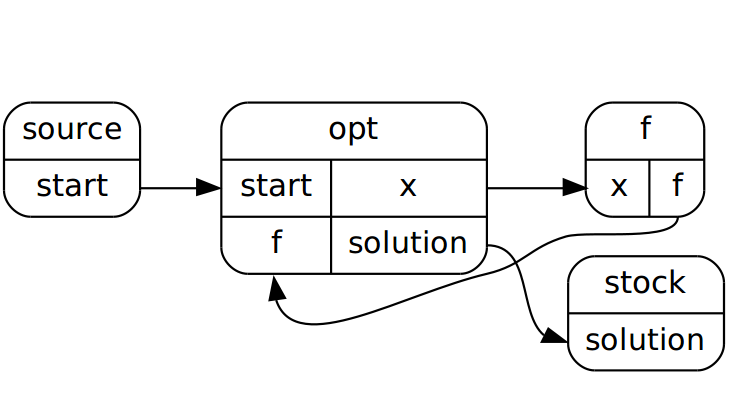
\includegraphics[width=0.5\textwidth]{optimization_workflow.png}
    \caption{Схема workflow для задачи оптимизации}
    \label{img:opt_wf}
\end{figure}

Так же в нашей модели мы учитываем , что в каждый момент времени у блок есть некоторое внутреннее состояние, которое может меняться от запуска к запуску. Тривиальный простер блока имеющего более одного внутреннего состояния - оптимизатор.



Перейдём к более формальному описанию блока в нашей модели.\\

Блок в нашей модели является единицей исполнения workflow, например, реализующей некоторую задачу  предметной области. 
Блок имеет интерфейс в виде входных  и выходных портов.
В нашем подходе блок описывается не детерминированным конечным автоматом.\\
 В нашем подходе , состояние блока в любой определённый момент времени характеризует, как блок будет реагировать на входные данные.

\begin{definition}{Определение: Конечный автомат блока} Конечным автоматом блока называется набор $M = (\Sigma, I, O, T, s_{0})$ , где
\begin{enumerate}
\item[-] $\Sigma$ -набор конечных состояния,
\item[-] $I$ - непустой набор доступных входных портов блока,
\item[-] $O$ - непустой набор доступных выходных портов блока,
\item[-] $I \bigcap O = \varnothing$ - 
\item[-] $s_{0} \in \Sigma$ - начальное состояние,
\item[-] $T: \Sigma \times (2^{I} \backslash \lbrace \varnothing \rbrace) \rightarrow  2^{\Sigma \times 2^{O}}$ отображение сопоставляющее каждому состоянию и набору входных портов набор состояний с соответствующим набором выходных портов.
\end{enumerate}
\end{definition}


\begin{figure}[here]
    \centering
    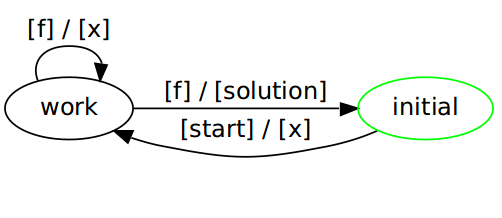
\includegraphics[width=0.5\textwidth]{optimizer_block.png}
    \caption{Граф состояний и переходов для оптимизирующего блока }
    \label{img:opt_wf}
\end{figure}

Где вершины графа - это возможные состояния. А рёбра - возможные переходы. Подписи на рёбрах показывают , какие порты необходимы для выполнения перехода, и данные по каким портам будут выписаны.




\subsection{Представление workflow}

 Мультиграф связей workflow $WFG =(A, D)$ состоит из набора блоков $A$ и набора связей D, соединяющих блоки через порты.
 При этом в состав набора блоков всегда $A$ входят два уникальных абстрактных блока \textit{Source} и \textit{Stock}, вводимых для задания точек запуска и завершения workflow.
 Формально связь $d \in D$ представима в виде четвёрки $(s, p_{s}, t, p_{t})$, где $s,t in A$ - идентификаторы входной и выходных блоков,  $ p_{s} \in out(s), p_{t} \in in(p)$ - выходной и входной порты соответствующих блоков. 
 
Отметим некоторые свойства, связанные со связями:
\begin{enumerate}
\item[-] Связь может быть установлена только между выходным портом одного блока и входным портом другого блока или самого себя.
\item[-] Связи могут быть построены как из одного выходного порта ко многим входным, так и из нескольких выходных в один входной порт.
\item[-]Обратим внимание, что если блок испускает сигнал по какому либо порту, то сигнал распространяется по всем связям исходящих, таким образом возможно порождаются конкурирующие потоки.
\item[-] Входные и выходные порты блоков могут оставаться неподключенными.
\end{enumerate} 
 
 
 
 
\subsection{Возможные ошибки при проектировании}
Для решения конкретной инженерной или научной  задачи должна быть составлена конкретная схема workflow.  Одной из целей работы было нахождение ошибок допущенных при составлении workflow.

Рассмотрим возможные ошибки.\\ 

Мы подразумеваем возможность асинхронной работы программных модулей на отдельных участках workflow. Следовательно то как и в многопоточных компьютерных программах возможно возникновение \textit{состояние гонки}(Race condition). 
В контексте нашей модели workflow состояние гонки бывает двух типов:
\begin{enumerate}
\item[•] Случай, когда на один входной порт приходят два сигнала одновременно.
\item[•] Когда на входные порты блока одновременно приходит такой набор сигналов, что что существует неоднозначность запуска.
Потенциально возможно в блоках, у которых есть состояния
$b = (S, \Sigma,\Lambda, T, s_{0});\\
 \exists s \in S , \exists in1, in2 \in 2^{\Sigma} :  T(s, in1) \neq \varnothing \bigwedge T(s, in2) \neq \varnothing$

Так же к ошибкам относится Голодание  - к концу работы workflow, остаются необработанные данные(сигналы)
\end{enumerate}

\section{Анализа модели workflow}


\begin{figure}[here]
    \centering
    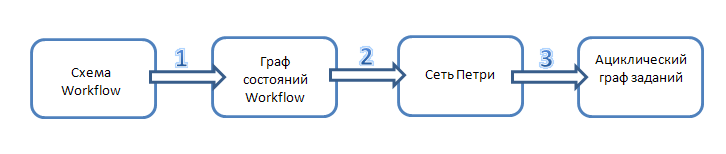
\includegraphics[width=\textwidth]{analys_plan.png}
    \caption{Граф состояний и переходов для оптимизирующего блока }
    \label{img:opt_wf}
\end{figure}

\begin{enumerate}
\item Модифицированный волновой алгоритм
\item Преобразование графа состояний workflow к виду сети Петри
\item Методы избавления от циклов и 
\end{enumerate}

Модифицированный волновой алгоритм
В работе был выработан алгоритм, моделирования работы workflow, являющийся некоторой модификацией волнового алгоритма.\\
Мы используем этот алгоритм для исследования поведения workflow и нахождения описанных ранее ошибок.

Мы считаем возможность возникновения состояние гонки ошибкой при построении workflow. И так как время работы каждого блока мы считаем априори неизвестным, то примем , что время работы каждого блока фиксировано и равно некоторомы значению T.


Для объяснения принципов работы данного алгоритма введём понятие состояния workflow.

Под состоянием workflow в определённый момент понимаем набор (BlockStates, WaveFront.\\
BlockStates - набор, состоящий из состояние каждого блока в составе workflow.\\

WaveFront - набор связей, по которым осуществляется передача данных в данный момент.


начальное состояние workflow (Initial Workflow State)	Начальным состоянием workflow будем называть то состояние в котором каждый блок находится в начальном состоянии, в соответствии с его конечным автоматом, и набор активных связей, состоит только из связей выходящих из блока Source.
В ходе работы модифицированного волнового алгоритма, начинающего работу из начального состояния, находятся новые возможные состояния workflow, и переход из одного состояния в новое, изображается в виде ребра на графе состояний.

На каждом шаге работы алгоритма, workflow переходит из одного состояние в другое, путём единовременного работы всех доступных для запуска блоков.


\begin{figure}[here]
    \centering
    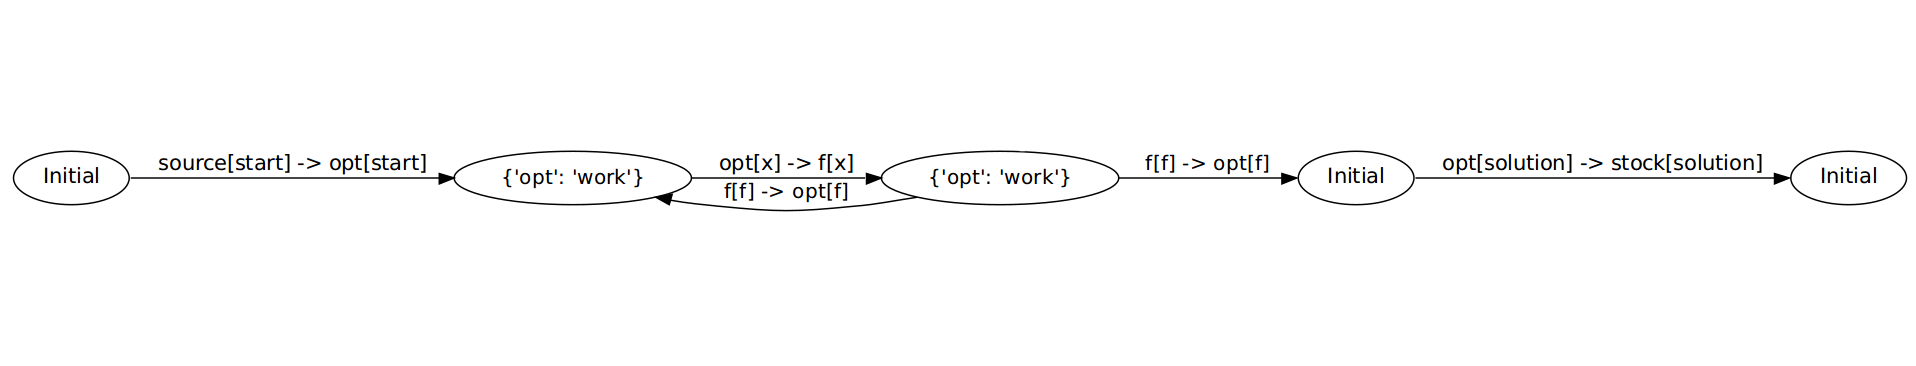
\includegraphics[width=\textwidth]{optimization_state_graph.png}
    \caption{Граф состояний и переходов для оптимизирующего блока }
    \label{img:opt_wf}
\end{figure}


Как правило, при моделировании workflow с помощью сетей петри, используют следующую нотацию:\\
задачи обозначаются переходами, а состояния системы местами.
В такой терминологии, несколько  
Как уже говорилось, при определении состояния workflow, одно состояние переходит в другое, посредством работы блока, группы непоследовательных блоков. Соответственно , наш граф состояний можно представить в виде сети петри, путём сопоставления , каждому состояния "места" в контексте сетей Петри, а каждому переходу из одного состоянию - соединение соответствующих мест через переход, олицетворяющий работу блока в 

\begin{figure}[here]
    \centering
    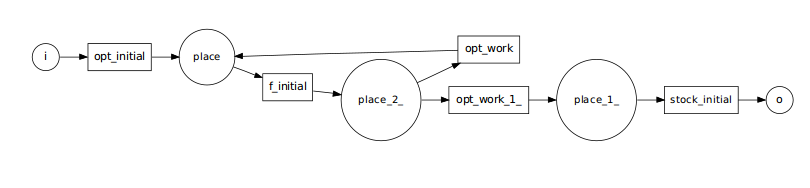
\includegraphics[width=0.8\textwidth]{optimization_petri_net.png}
    \caption{Граф состояний и переходов для оптимизирующего блока }
    \label{img:opt_wf}
\end{figure}




Возвращаясь к поставленной задаче, мы хотим найти стратегию запуска workflow в распределённой вычислительной среде.
В этом контексте это означает распределить блоки по узлам.
\\ Опишем некоторые ограничение, вводимые для упращения поставленной задачи.
\begin{enumerate}
\item[•] Считаем , что блоки не переносимы с одного узла на другой.
\item[•] На одном узле может быть запущено несколько блоков, но работать они могут только последовательно.
\end{enumerate}



\end{document}